\chapter{User Experience Evolution}

\section{Early Electronic Computers}
Computers and how we use them have changed dramatically as each generation is introduced to faster and better machines. How we interact with computers has changed drastically since the first electronic computers in the mid-1900s.

\begin{wrapfigure}{r}{0.5\textwidth}
  \begin{center}
    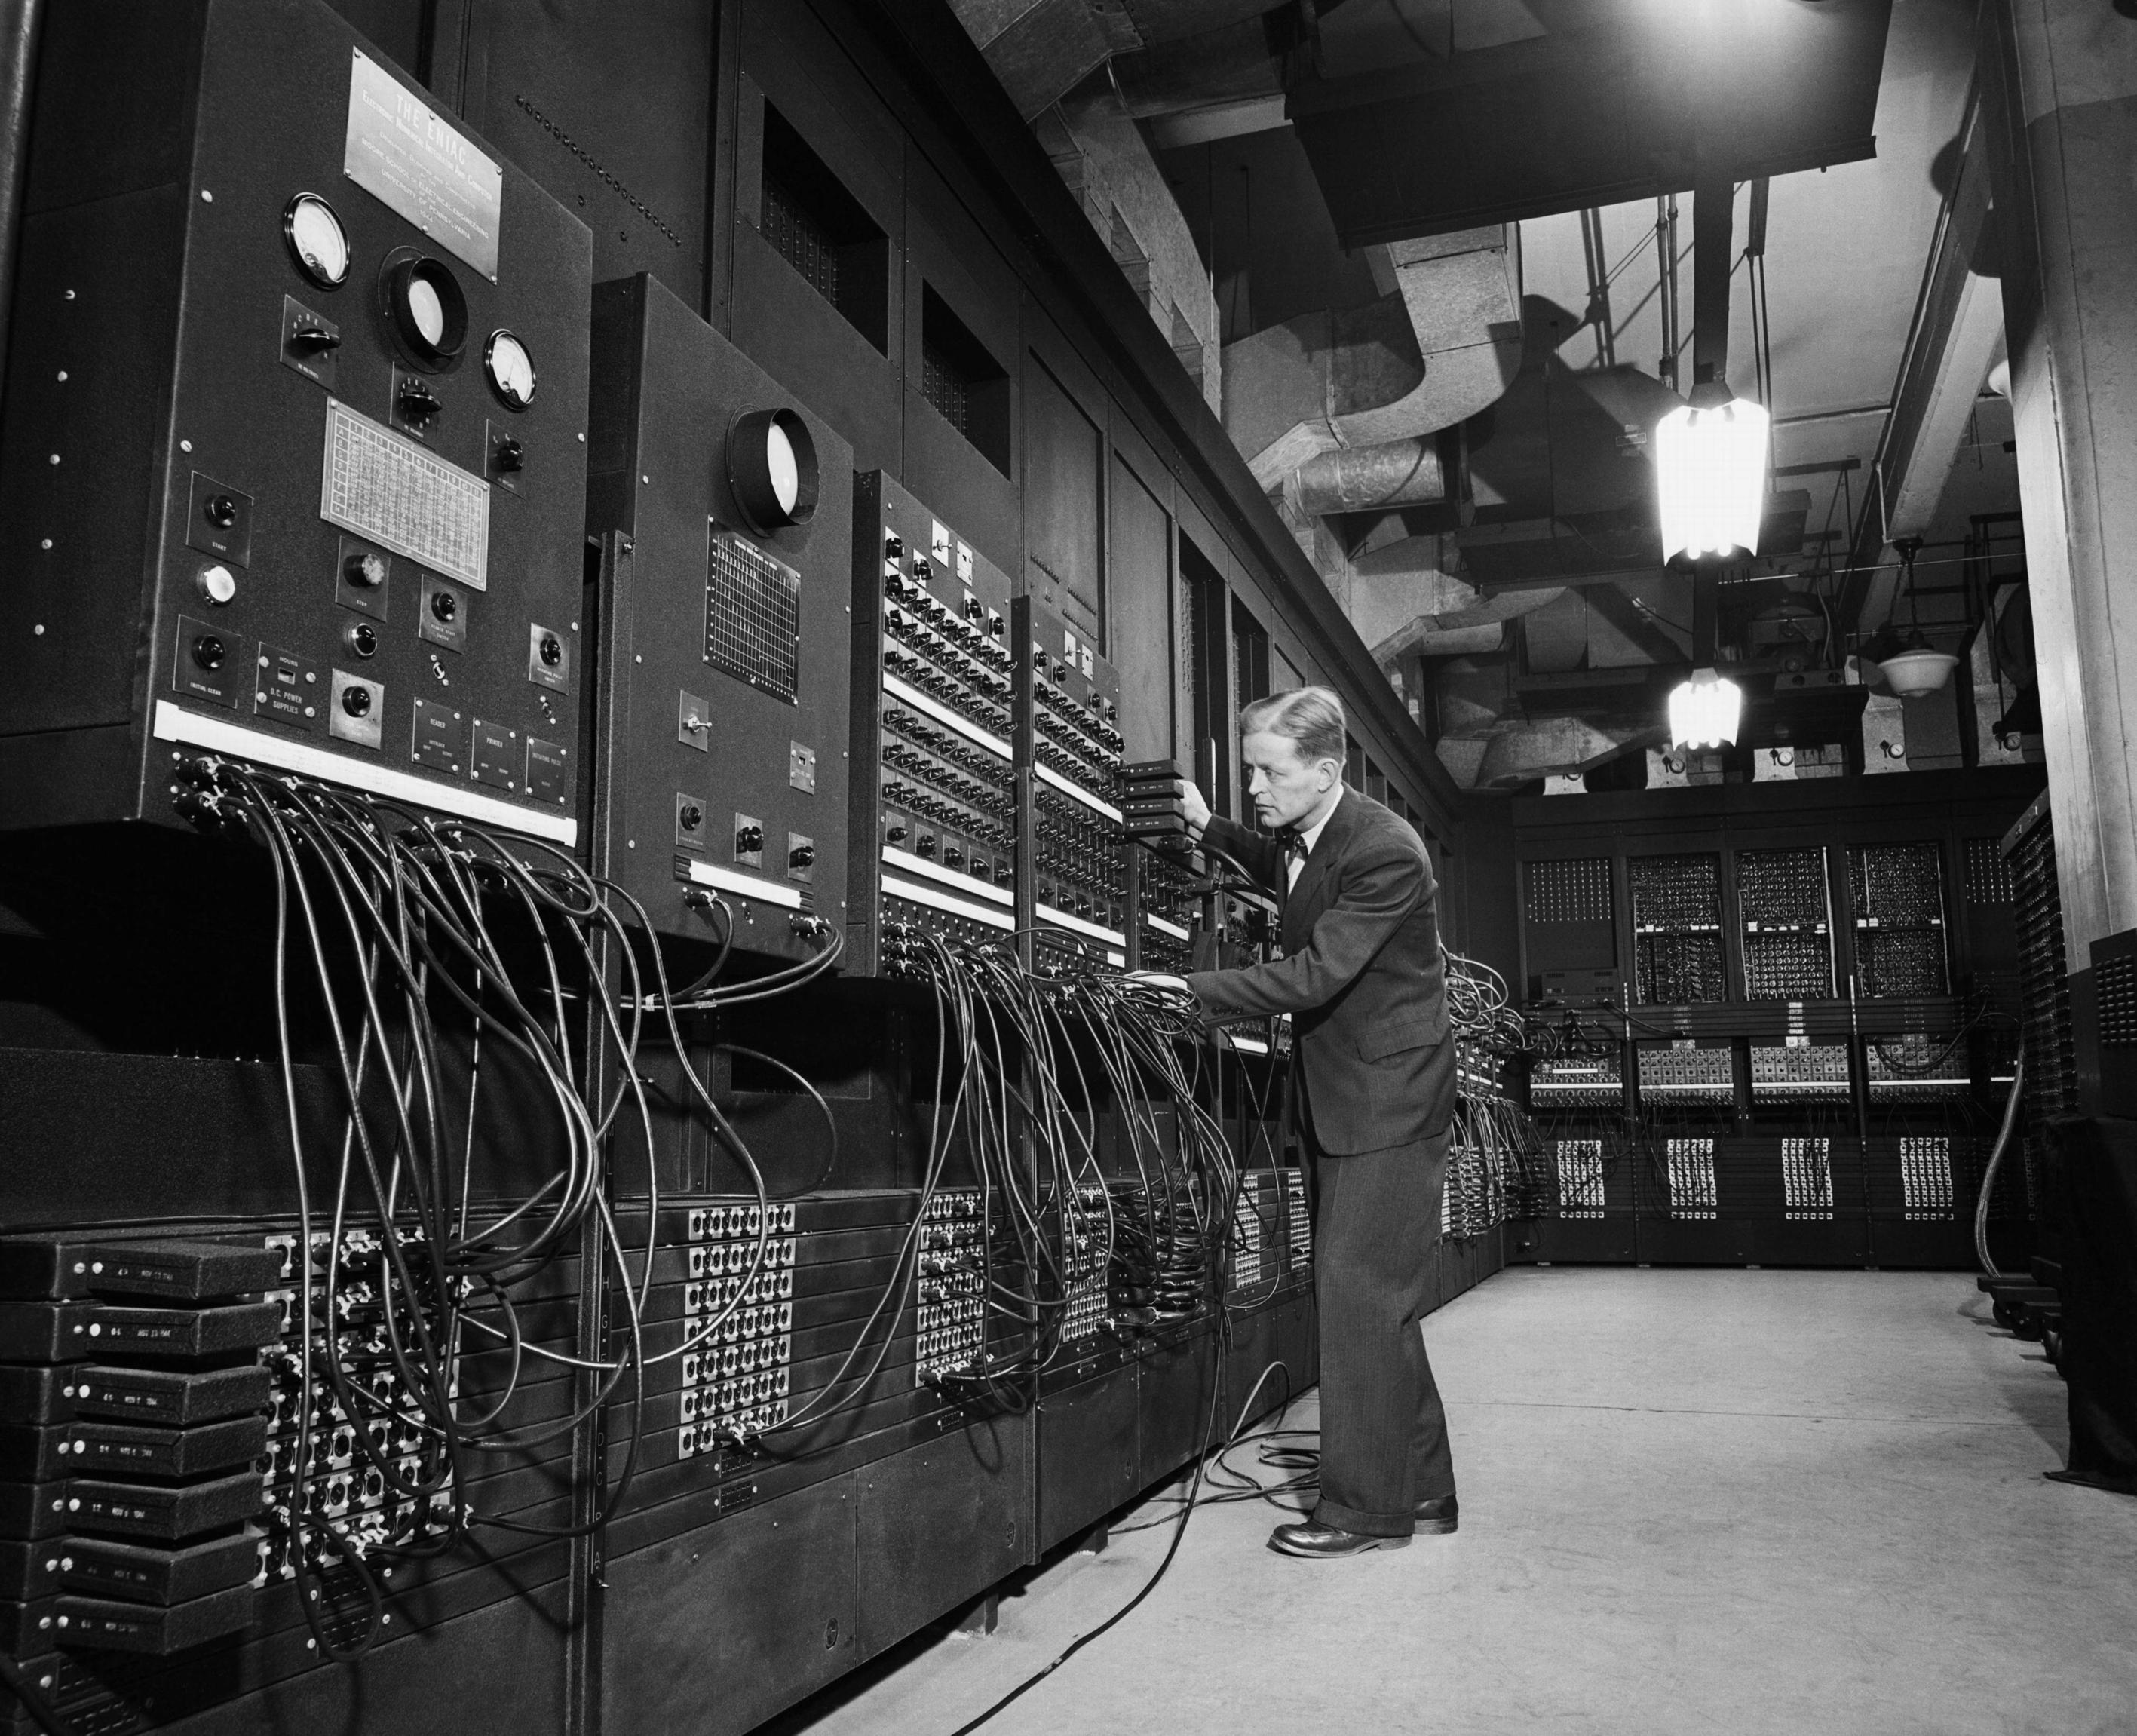
\includegraphics[width=0.48\textwidth]{img/eniac.jpg}
  \end{center}
  \caption{ENIAC}
\end{wrapfigure}

Early electronic computers such as the ENIAC (Electronic Numerical Integrator and Computer). \cite{eniac} The ENIAC was the first general purpose computer, this meant it could solve many problems as it could be programmed. The ENIAC was the first real step in user interaction with a computer, although the user had to have knowledge of the machine first, they could still operate it using over 3,000 switches and wires which could change how the machine made calculations. \cite{eniac} Although a primitive method of user interaction with a machine, it was the first 'modern' computer which the user had some control over its operation and change its operation by interaction.

Moving on from the ENIAC new computers were built with observations on how to improve over the ENIAC. Machines like the Manchester Baby \cite{manchesterbaby} allowed programs to be saved which was a huge leap in user intractable computers. Once a program was created by a programmer of the machine they could be saved and used again at a later date. This was a big step over the ENIAC where it took time to reprogram the machine each time they wanted to compute a specific task.

\begin{wrapfigure}{r}{0.5\textwidth}
  \begin{center}
    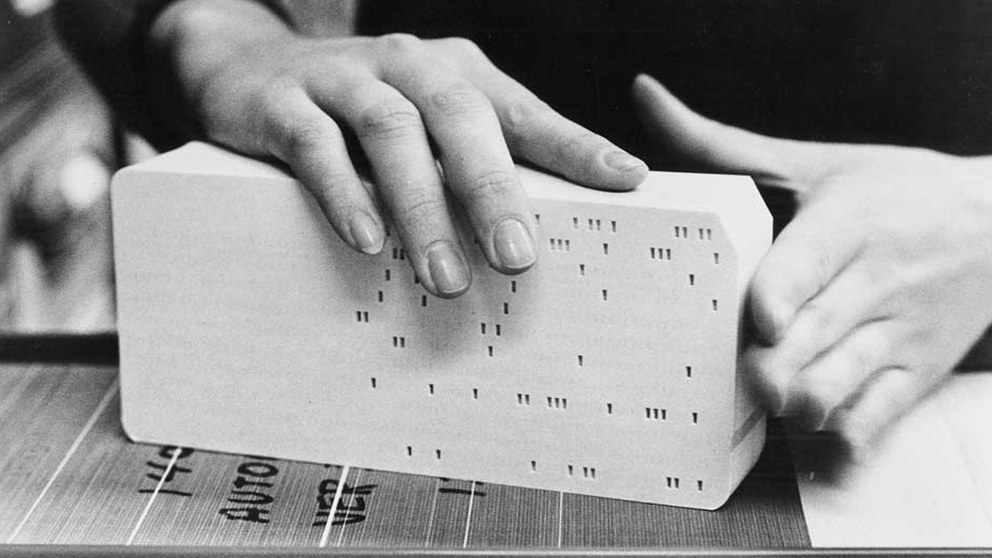
\includegraphics[width=0.48\textwidth]{img/punchcard.jpg}
  \end{center}
  \caption{Punch card}
\end{wrapfigure}

As computers advanced and went from large machines that took up an entire room to smaller and smaller devices. During the 1960s to early 1970s computers started being more accessible by university's and businesses. These general purpose computers allowed the user to interact with the computer using punch cards. \cite{punchcard} Punch cards have been along since long before the computer emerging in the late 1800s. \cite{punchcard} These punch cards allowed computers to be more easily accessible by a large amount of people. Students would be able to make program with these punch cards and use them to give the instructions to the computer. Businesses would also use these punch cards to calculate business related queries.

\section{Home Computers}

\begin{wrapfigure}{r}{0.5\textwidth}
  \begin{center}
    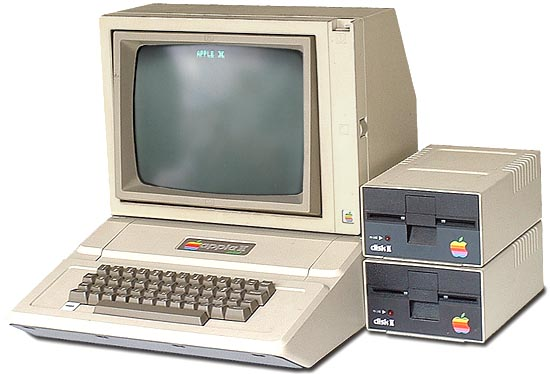
\includegraphics[width=0.48\textwidth]{img/appleii.jpg}
  \end{center}
  \caption{Apple II}
\end{wrapfigure}

Modern computers started when the computer entered the home. \cite{homecomputers} These home computers started in the last 1970s with the Apple II, TRS-80 Model I and the Commodore PET. These three home computers created enough competition to keep prices low enough for many users to start getting into the first generation of home computers. These home computers were the first real leap for users interacting with computers. These computers used DOS. \cite{dos} DOS (Disk Operating System) was designed to make interaction with a computer easier for users who never interacted with computers before this point. These computers also had a Keyboard to make interaction with the computer easier. With the keyboard and a basic OS (Operating System) the home computer was a great success, and turned the computer to something that only organizations used to a more personal item.

These new computers allowed users to buy software from vendors that would add extra functionality to their computer through the floppy disk drive. The same floppy disk drive could be used to save data to floppy disks. This allowed user to easily transfer data between machines.

Later home computer improved in hardware, software and their operating system. Operating systems improved dramatically after hardware manufacturers moved away from DOS. Operating systems such as Windows 3/3.1 and System 1-7 (Classic Mac OS) made user interaction with the home computer easier and allowed multi-tasking by using "tabs" which the user could flick between. These tabs were controlled with a new technology for the time, the computer mouse. 

\begin{wrapfigure}{r}{0.5\textwidth}
  \begin{center}
    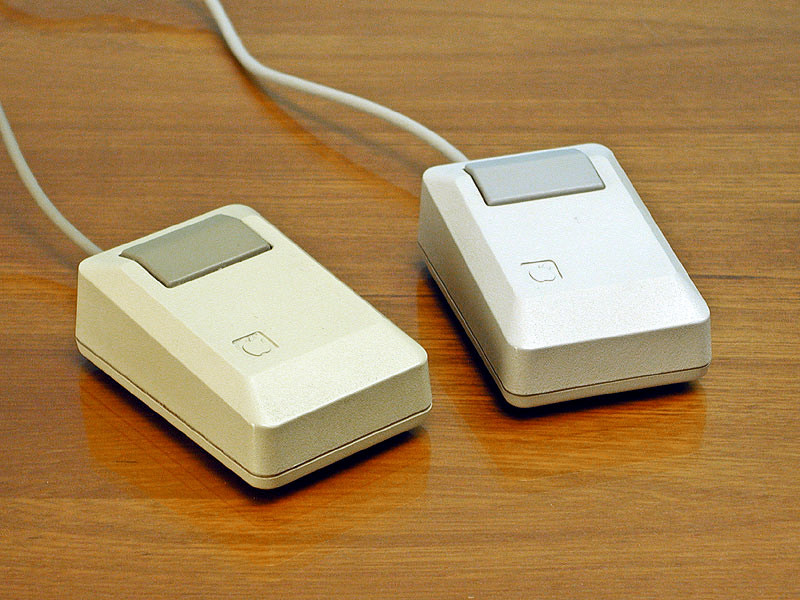
\includegraphics[width=0.48\textwidth]{img/mouse.jpg}
  \end{center}
  \caption{Apple II}
\end{wrapfigure}

The computer mouse was a perfect addition to the home computer as it allowed more refined selection to the new OSs introduced by the newer models of home computers. The mouse paired with the keyboard allowed greater control over computers that couldn't be achieved by just a keyboard. 

Over the years operating systems would improve and add more and more features to improve user interact-ability. A great example of the modern operating system is Microsoft. Microsoft have become the largest OS provider to hardware manufacturers. Microsoft have released an OS for nearly every device in every situation. OSs such as Windows 10 for home computers, Windows Phone for mobile phones, Windows Server 2019 for servers and legacy OSs such as windows Embedded Compact for systems such as cash registers. Windows has stayed in the OS market by staying relevant and innovating.

With the latest OSs such as Windows 10 users can now use voice controls via Cortana. This was a very important addition for people who are blind or visual impaired. Cortana allows the users to search the internet, launch applications and generally help the users.

\section{Touch devices}

\begin{wrapfigure}{r}{0.5\textwidth}
  \begin{center}
    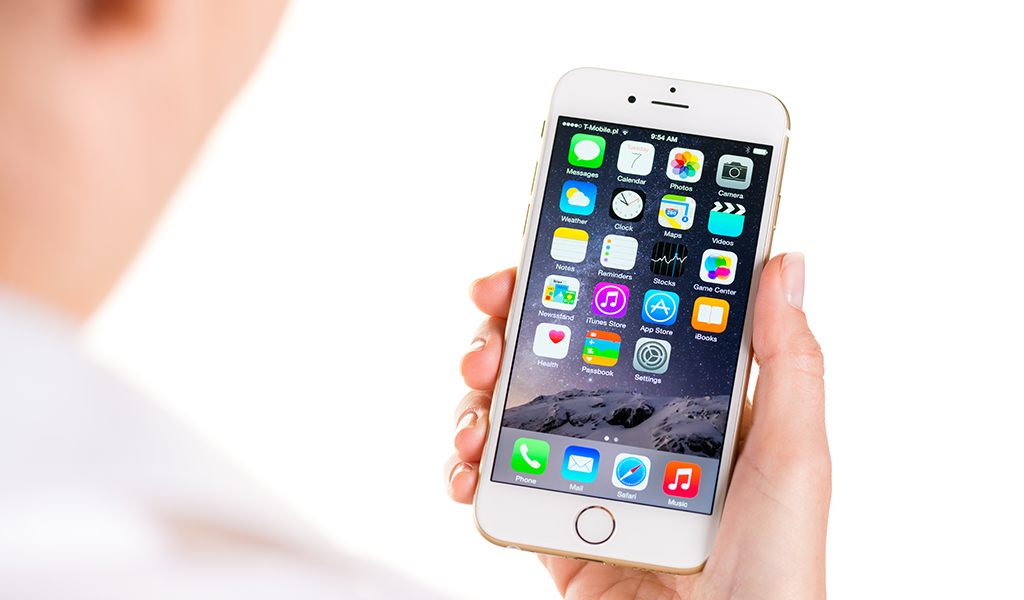
\includegraphics[width=0.48\textwidth]{img/smartphone.jpg}
  \end{center}
  \caption{Modern Smart phone}
\end{wrapfigure}

As computers got smaller and cheaper it lead to companies like Samsung and Apple developing new mobile phones called smart phones. These phones moved away from the traditional full button interface. These smart phones had touch screens which made more room for the screen, which increased its usability.

Modern smart phones have used this touchscreen capability to the next level by adding finger print reader into them and adding gesture controls while the phone is off. The user can do gestures such as a two finger swipe down to pause music, or an arrow gesture to play the next song. Face unlock as also become more popular moving further away from directly interacting with the device.
